\documentclass[10pt,twocolumn]{article} 
\usepackage{latex8}
%\usepackage{pslatex}

\usepackage{amsmath}
\usepackage{times}
\usepackage{comment}
\usepackage{amssymb}
\usepackage{amsmath}
\usepackage{ifthen}
\usepackage{fancyvrb}
\usepackage{alltt}
\usepackage{multirow}
\usepackage{xspace}
\usepackage{graphicx}
\usepackage{url}
\usepackage{color} 
\urlstyle{sf}
\usepackage{makeidx}
\usepackage{cite}
\usepackage{url}
\usepackage{rotating}
\usepackage{multirow}
\usepackage[figure]{algorithm2e}
\usepackage{relsize}

\newcommand{\TechReport}[1]{}
\newcommand{\ConfPaper}[1]{#1}
\newboolean{hidecomments}
\setboolean{hidecomments}{false}
\ifthenelse{\boolean{hidecomments}}
{\newcommand{\nb}[2]{}}
{\newcommand{\nb}[2]{
    \fbox{\bfseries\sffamily\scriptsize#1}
    {\sf\small$\blacktriangleright$
      {#2} $\blacktriangleleft$}}}
\newcommand\John[1]{\nb{John}{#1}}
%\newcommand\Danny[1]{\textbf{Danny: {#1}}} 
\newcommand\Danny[1]{\nb{Danny}{#1}}
%\newcommand\Feedback[1]{\textcolor{red}{#1}}
\newcommand\Feedback[1]{#1} 
\newcommand\todo[1]{\fbox{\bfseries\sffamily\scriptsize TODO: #1}}
\newcommand{\tool}{\begin{scriptsize}\textsc{Concurrencer}\end{scriptsize}\xspace}
\newcommand{\toolx}{{\smaller\textsc{Concurrencer}}\xspace}
\newenvironment{CodeOut}{\begin{scriptsize}}{\end{scriptsize}}
\newcommand{\code}[1]{\begin{smaller}\texttt{#1}\end{smaller}}
\newcommand{\codex}[1]{{\smaller\texttt{#1}}\xspace}
\newcommand{\myParagraph}[1]{\textbf{#1}}
\newcommand{\HalfWidth}{.40\columnwidth}
\newcommand{\FullWidth}{.95\columnwidth}
\newcommand{\MaxWidth}{\columnwidth}
\newcommand{\ShorterWidth}{.92\columnwidth}
\newcommand{\LongerWidth}{1.08\columnwidth}
\newcommand{\LOCSavedInForkJoinTask}{{302}\xspace}
\newcommand{\humanOmissions}{{41}\xspace}
\newcommand{\LOCchangedTool}{{1004}\xspace}
\newcommand{\LOCchangedManually}{{1019}\xspace}
\newcommand{\LOCNeedChangeManually}{{15}\xspace}
\newcommand{\ConvertToAtomicInteger}{{\begin{smaller}\begin{smaller}\textsc{Convert Int to AtomicInteger}\end{smaller}\end{smaller}}\xspace}
\newcommand{\ConvertToConcurrentHashMap}{{\begin{smaller}\begin{smaller}\textsc{Convert HashMap to ConcurrentHashMap}\end{smaller}\end{smaller}}\xspace}
\newcommand{\ConvertToForkJoinTask}{{\begin{smaller}\begin{smaller}\textsc{Convert Recursion to ForkJoinTask}\end{smaller}\end{smaller}}\xspace}
\newcommand{\ConvertToAtomicIntegerx}{{\smaller\smaller\textsc{Convert Int to AtomicInteger}}\xspace}
\newcommand{\ConvertToConcurrentHashMapx}{{\smaller\smaller\textsc{Convert HashMap to ConcurrentHashMap}}\xspace}
\newcommand{\ConvertToForkJoinTaskx}{{\smaller\smaller\textsc{Convert Recursion to ForkJoinTask}}\xspace}
%% Define a new 'leo' style for the package that will use a smaller font.
\makeatletter
\def\url@leostyle{%
  \@ifundefined{selectfont}{\def\UrlFont{\sf}}{\def\UrlFont{\small\ttfamily}}}
\makeatother
%% Now actually use the newly defined style.
\urlstyle{leostyle}

\newcommand{\ConcurrentHashMap}{\codex{Con\-cur\-rent\-Hash\-Map}}

% Add line between figure and text
\makeatletter
%\nocaptionrule %remove the line above the caption %%ACM
\def\topfigrule{\kern3\p@ \hrule \kern -3.4\p@} % the \hrule is .4pt high
\def\botfigrule{\kern-3\p@ \hrule \kern 2.6\p@} % the \hrule is .4pt high
\def\dblfigrule{\kern3\p@ \hrule \kern -3.4\p@} % the \hrule is .4pt high
\makeatother

\makeatletter
\newcommand{\captionfont}{\normalfont}
\long\def\@makecaption#1#2{
   \vskip \baselineskip
   \setbox\@tempboxa\hbox{\captionfont{#1: #2\strut}}
   \ifdim \wd\@tempboxa >\hsize % IF longer than one line:
       {\captionfont\noindent\parbox{\hsize}{#1: #2\strut}}\par     %   THEN set as ordinary paragraph.
     \else                      %   ELSE  center.
       \hbox to\hsize{\hfil\box\@tempboxa\hfil}
   \fi}
\makeatother

\hyphenation{Con-cur-rent-Hash-Map Para-Scope Fork-Join-Task
  max-Sum-Con-sec-u-tive Hash-Map}


%------------------------------------------------------------------------- 
% take the % away on next line to produce the final camera-ready version 
\pagestyle{plain}
%------------------------------------------------------------------------- 
\begin{document}

\title{Refactoring Sequential Java Code for Concurrency via Concurrent
Libraries}

\author{Danny Dig, John Marrero, Michael D. Ernst\\
Massachusetts Institute of Technology\\ Computer Science and Artificial
Intelligence Laboratory \\ \{dannydig,marrero,mernst\}@csail.mit.edu\\
}

\maketitle
\thispagestyle{empty}

\begin{abstract}
Parallelizing existing sequential programs to run efficiently on multicores is
hard.  The Java 5 package
\code{java.util.concurrent} (\code{j.u.c.})\ supports writing concurrent
programs: much of the complexity of writing thread-safe and scalable programs is hidden in the
library. To use this package, programmers still need to reengineer
existing code. This is \emph{tedious} because it requires changing many lines
of code, is \emph{error-prone} because programmers can use the wrong APIs,
and is \emph{omission-prone} because programmers can miss opportunities to
use the enhanced APIs.

This paper presents our tool, \tool, that enables programmers to refactor
sequential code into parallel code that uses \Feedback{three} \code{j.u.c.}\
concurrent utilities. \tool does not require any program annotations. Its
transformations span multiple, non-adjacent, program statements. A
find-and-replace tool can not perform such transformations, which require
program analysis. Empirical evaluation shows that \tool refactors code
effectively: \tool correctly identifies and applies transformations that some
open-source developers overlooked, and the converted code exhibits good speedup.


%Abstract Submission
% Parallelizing existing sequential programs to run efficiently on multicores is
% hard. Java 5's java.util.concurrent (j.u.c.)\ package supports writing concurrent programs: the complexity of writing threads-safe and scalable programs is hidden in the library. To use this package, programmers need to reengineer existing code. This is tedious because it requires changing many lines of code, is error-prone because programmers can use the wrong APIs, and is omission-prone because programmers can miss opportunities to use the enhanced APIs.
% 
% This paper presents our tool, Concurrencer, which enables programmers to refactor
% sequential code into parallel code that uses the j.u.c.\ package. Concurrencer does not require any program annotations, although the transformations are involved: they span over several program statements and use custom program analysis. A find-and-replace tool cannot perform such transformations. Empirical evaluation shows that Concurrencer is effective: Concurrencer correctly applies transformations that open-source developers overlooked, and the converted code exhibits good speedup.


\end{abstract}


%------------------------------------------------------------------------- 
\section{Introduction}

% \Danny{Should I recast the problem as a trade-off between safety and liveness,
% rather than safety vs. scalability?}

% The problem: multicores are here
Users expect that each new generation of computers runs their programs faster than
the previous generation. The computing hardware industry's shift to
multicore processors demands that programmers find and exploit
parallelism in their programs, if they want to reap the same performance
benefits as in the past.

% The challenge: parallelize sequential applications
It is arguably easier to design a program with
concurrency in mind than to retrofit concurrency later~\cite{Lea:CPJ99,
Goetz:JCP06}. However, most desktop programs were not designed to be concurrent, so
programmers have to refactor existing sequential programs for concurrency. It
is easier to retrofit concurrency than to rewrite, and retrofitting is often
possible.


% Concrete challenge: thread-safety and scalability
The dominant paradigm for concurrency in desktop programs is multithreaded
programs where shared-memory accesses are protected with locks. However,
programming with locks is error-prone: too many locks can slow
down or even deadlock an application, while too few locks result in data races. 


% Java.util.concurrent class library
Java 5's \code{java.util.concurrent} (\code{j.u.c.})\ package supports writing
concurrent programs. Its \code{Atomic*} classes offer thread-safe, lock-free programming over 
single variables. Its thread-safe abstract data types (e.g.,
\ConcurrentHashMap) are optimized for scalability. 

Java 7 will contain the \emph{ForkJoinTask} framework~\cite{Lea:jsr166y, DougLea'00:forkJoinFramework} for
fine-grained parallelism. Many computationally-intensive problems take the form of recursive
\emph{divide-and-conquer}. Classic examples include sorting (e.g., mergesort,
quicksort), searching, and many data structure or image processing algorithms.
Divide-and-conquer algorithms are good candidates for parallelization since the
subproblems can be solved in parallel.

%The conversion task is still error-prone
In order to benefit from Java's concurrent utilities and frameworks,
the Java programmer needs to refactor existing code. This is \emph{tedious}
because it requires changing many lines of code. For example, the developers of
six widely used open-source projects changed \LOCchangedManually lines when
converting to use \Feedback{\code{AtomicInteger} and \ConcurrentHashMap}.
Second, manual refactoring is \emph{error-prone} because the programmer can choose the wrong APIs among
slightly similar APIs. In the above-mentioned projects, the programmers four
times mistakenly used \code{getAndIncrement} API methods instead of
\code{incrementAndGet}, which can result in off-by-one values. Third, manual
refactoring is \emph{omission-prone} because the programmer can miss
opportunities to use the new, more efficient API methods. In the same projects,
programmers missed \humanOmissions such opportunities.

% This paper presents \tool and three automated refactorings:

This paper presents our approach for incrementally retrofitting parallelism
through a series of behavior-preserving program transformations, namely
refactorings. Our tool, \tool, enables Java programmers to refactor their
sequential programs to use \code{j.u.c.}\ utilities: the programmer selects
shared data and a target refactoring, and \tool analyzes all accesses to the shared data and applies the 
transformation. Ultimately, it is the programmer's responsibility to identify
all shared data and target it with the refactorings.
% \Comment{by describing the process, and that the programmer is
% responsible for selecting the shared data and the refactoring, I'm addressing
% Reviewer1's comment on the unguaranteed thread-safety: the process is not
% automatic (i.e., tool finds all shared data and makes it thread-safe), but
% it requires human intervention}


% Enumerate the three refactorings and why we chose them
Currently, \tool supports three refactorings: (i)
\ConvertToAtomicInteger, (ii) \ConvertToConcurrentHashMap, and
(iii) \ConvertToForkJoinTask. Although these are not all the refactorings
that one needs for parallelization, the first two refactorings are among the
most commonly used in practice, as evidenced by our
study~\cite{Dig'08:studyOfConcurrentTransformations} of how open-source
developers parallelized five projects. These three refactorings are are a
proof-of-concept for the toolset that one needs for parallelization.
% \Comment{this addresses reviewer's concern that these are not all the
% refactorings that one would ever need for parallelization.}

% ConvertToAtomicInteger
The first refactoring, \ConvertToAtomicInteger, enables a programmer to
convert an \code{int} field to an \code{AtomicInteger}, a utility
class that encapsulates an \code{int} value. The encapsulated field can be
safely accessed from multiple threads, without requiring any synchronization
code. Our refactoring replaces all field accesses with calls to
\code{AtomicInteger}'s thread-safe APIs. For example, it replaces expression
\code{f = f + 3} with \code{f.addAndGet(3)} which executes atomically. 


% ConvertToConcurrentHashMap 
The second refactoring, \ConvertToConcurrentHashMap, enables a programmer
to convert a \code{HashMap} field to \ConcurrentHashMap, a thread-safe,
highly scalable implementation for hash maps. Our refactoring replaces map
updates with calls to the APIs provided by \ConcurrentHashMap. For
example, a common update operation is (i) check whether a map contains a
certain $key$, (ii) if not present, create the value object, and (iii) place
the value in the map. \tool replaces such an updating pattern with a call 
to \ConcurrentHashMap's \code{putIfAbsent} which
\emph{atomically} executes the update, without locking the entire map. 

The third refactoring, \ConvertToForkJoinTask, enables a
programmer to convert a sequential divide-and-conquer algorithm to a parallel
algorithm. The parallel algorithm solves the subproblems in parallel
using the ForkJoinTask framework. Using the skeleton of the sequential
algorithm, \tool extracts the sequential computation into tasks that run in
parallel and dispatches these tasks to the ForkJoinTask framework.

Typically a user would first make a program thread-safe, i.e., the program has 
the same semantics as the sequential program even when executed under multiple 
threads, and then make the program run concurrently under multiple threads. 
\tool supports both kinds of refactorings. The first two refactorings 
are ``enabling transformations'' that make a program thread-safe. The 
third refactoring makes a sequential program run concurrently.

The transformations performed by these refactorings require matching certain
code patterns which can span several non-adjacent program statements, and they
require program analysis which uses data-flow information. Such transformations
can not be safely executed by find-and-replace.

%While it is possible to transform the code manually, a
% human can miss such patterns.
 
%Contributions
This paper makes the following contributions:
\begin{itemize}
  \item {\textbf {Approach.}} We present an approach for
  retrofitting parallelism into sequential applications through
  automated, but human-initiated, program transformations. Since the
  programmer is expert in the problem domain, she is the one most qualified to
  choose the code and the program transformation for parallelizing the code.
  
  \item {\textbf {Tool.}} We implemented three transformations for using
  thread-safe, highly scalable concurrent utilities and frameworks. Our
  tool, \tool, is conveniently integrated within Eclipse's refactoring engine.
  Since \tool is neither complete, nor sound, it can not guarantee absolute
  thread-safety. Nevertheless, it is safer and faster than making all the
  changes by hand. \tool can be downloaded from:  \\
   \code{http://refactoring.info/tools/Concurrencer}   
  
  \item {\textbf {Empirical Results.}} We used \tool to refactor the same
  code that the open-source developers of 6 popular projects converted to 
  \code{AtomicInteger} and \ConcurrentHashMap. By comparing the manually
  vs. automatically refactored output, we found that \tool applied all the
  transformations that the developers applied. Even more, \tool avoided
  the errors which the open-source developer \emph{committed}, and \tool
  identified and applied some transformations that the open-source developers
  \emph{omitted}. We also used \tool to parallelize 6 divide-and-conquer
  algorithms. The parallelized algorithms perform well and exhibit good speedup. These
  experiences show that \tool is useful.
\end{itemize}



%------------------------------------------------------------------------- 
%--------------------------------------------
\section{Convert Int to AtomicInteger}

\subsection{AtomicInteger in Java}
The Java 5 class library
offers a package \code{j.u.c.atomic} that
supports \emph{lock-free} programming on \emph{single} variables. 

The package contains wrapper classes over primitive variables, for example,
an \code{AtomicInteger} wraps an \code{int} value. The main advantage
is that update operations execute atomically, without blocking. 
%For example,
% \code{AtomicInteger} provides an API method \code{addAndGet(int delta)} that
% atomically adds the given delta to the current value. 
Internally, \code{AtomicInteger} employs efficient machine-level
atomic instructions like \emph{Compare-and-Swap} that are available on 
contemporary processors. Using \code{AtomicInteger}, the programmer
gets both \emph{thread-safety} (built into the \code{Atomic} classes) and
\emph{scalability} (the lock-free updates eliminate lock-contention under heavy
accesses~\cite{Goetz:JCP06}).

% However, \code{Atomic} classes are not meant as a general replacement for
% locking. One can use them only when the critical sections for an object require
% updates to a \emph{single} variable. Sometimes an object needs to maintain an
% invariant involving more than one variable (e.g., a \code{ValueRange} object
% needs to ensure that its \code{max} int field is always greater than its
% \code{min} int field). In such cases the programmer cannot use an
% \code{AtomicInteger} to maintain a \emph{multi-variable} invariant, but
% needs to use a lock around code which updates those variables together.
% 
% Additionally, atomic classes are not a general purpose replacement for their
% related classes. \code{AtomicInteger} is \emph{mutable} while its equivalent
% \code{Integer} class is \emph{immutable}. Therefore, an \code{AtomicInteger}
% does not define \code{hashCode} and \code{equals} methods.  

% With all the restrictions on \code{Atomic} classes, why would a programmer use
% them? Using \code{Atomic} classes, the programmer gets both \emph{thread-safety}
% (built-in the \code{Atomic} classes) and \emph{scalability} (the lock-free
% updates reduce lock-contention under heavy accesses~\cite{Goetz:JCP06}).
 
 
 %\usepackage{graphics} is needed for \includegraphics
\begin{figure}[tp]
  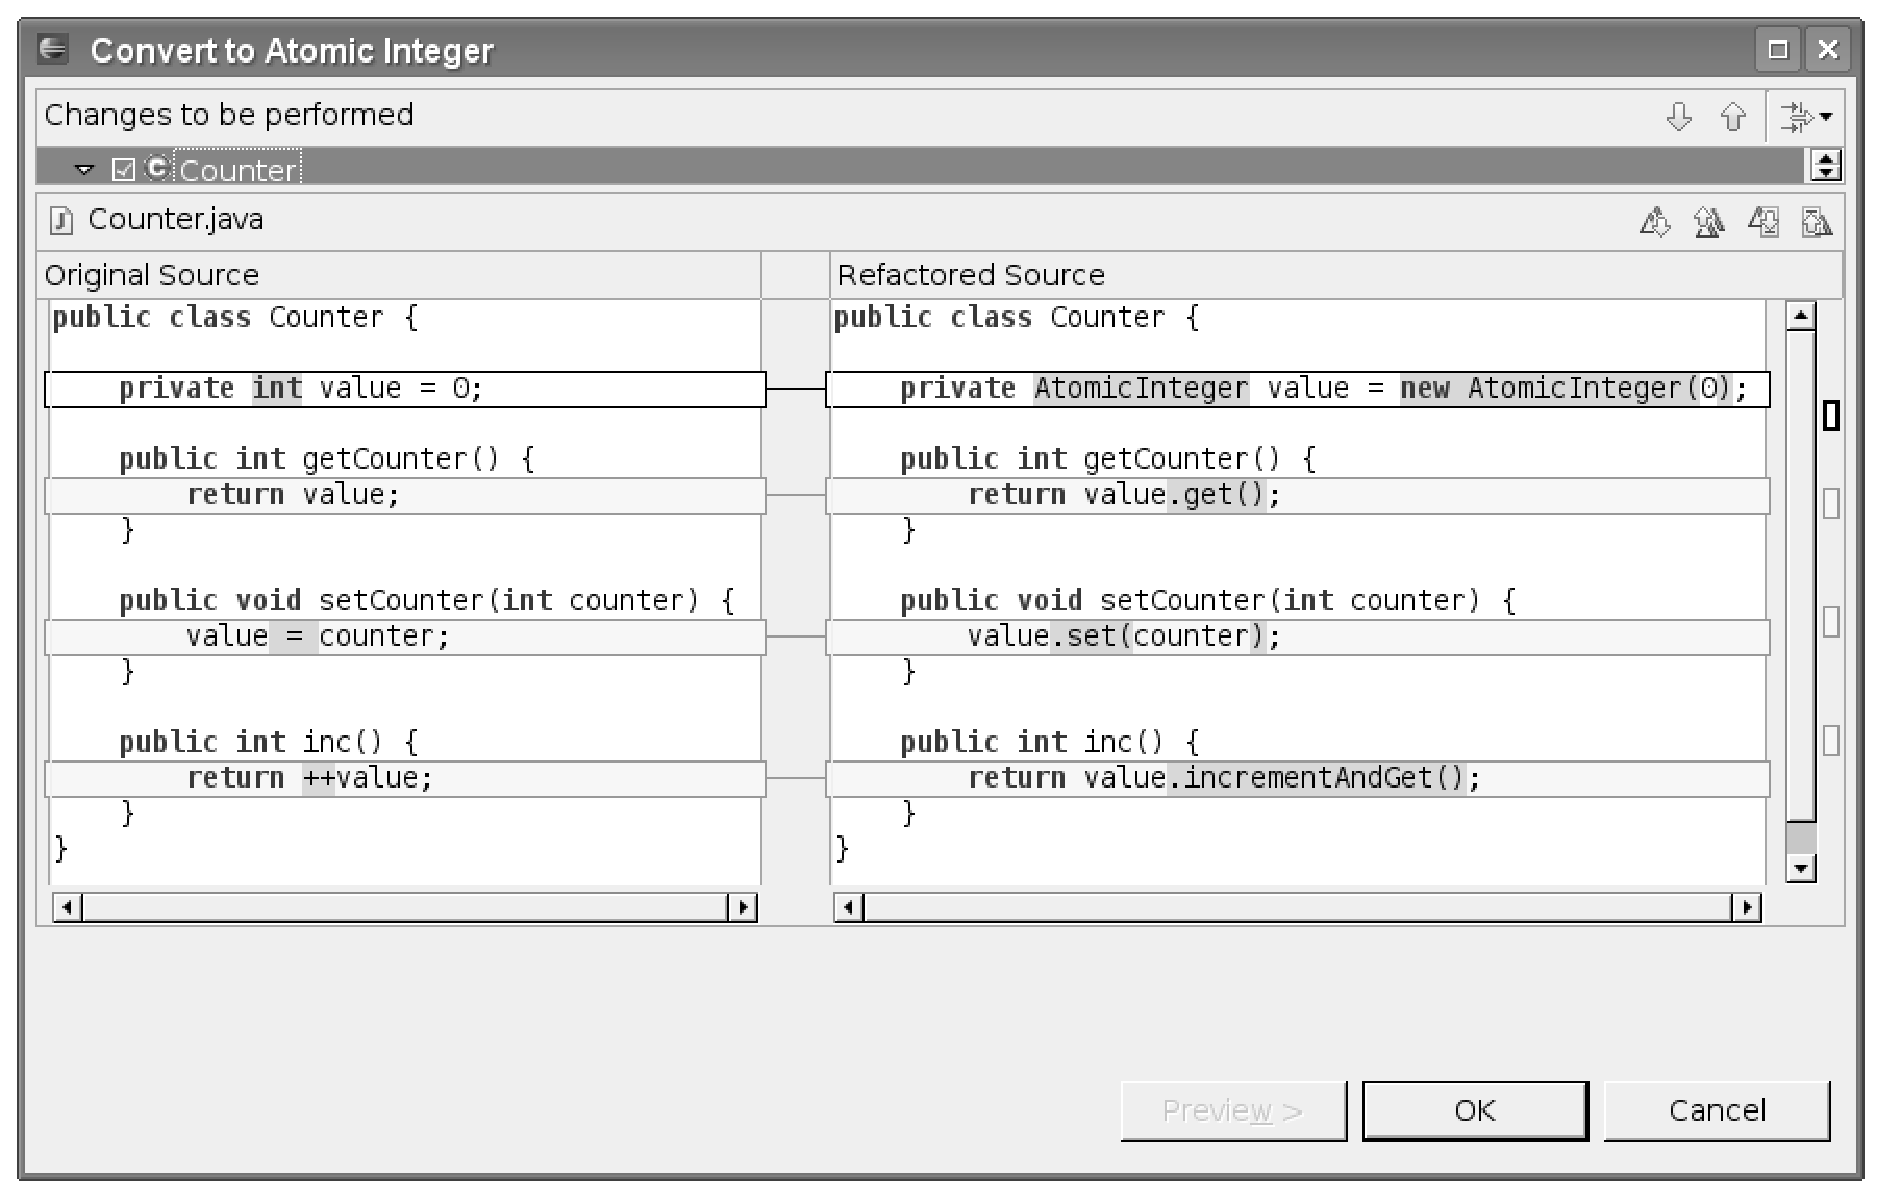
\includegraphics[width=\columnwidth]{./figs/ConvertToAtomicInteger}\
  \caption{Using \toolx to convert an \codex{int} to \codex{AtomicInteger} in Apache Tomcat.
The screenshot shows a preview of the changes.}
  \label{fig:CounterExample}
\end{figure}


\subsection{Code Transformations}
% \begin{figure*}[t]
% \begin{CodeOut}
% \begin{tabular}{@{}l|l@{}}
% \begin{minipage}[t]{\FullWidth}
% \begin{verbatim}
% // before refactoring
% public class Counter {
% 
%  private int value = 0;
%         
%  public int getCounter() {
%   return value;
%  }
%         
%  public void setCounter(int counter) {
%   value = counter;
%  }
%         
%  public int inc() {
%   return ++value;
%  }
% }
% \end{verbatim}
% \end{minipage}
% &
% \begin{minipage}[t]{\FullWidth}
% \begin{verbatim}
% // after refactoring
% public class Counter {
%  
%  private AtomicInteger value = new AtomicInteger(0);
%         
%  public int getCounter() {
%   return value.get();
%  }
%         
%  public void setCounter(int counter) {
%   value.set(counter);
%  }
%         
%  public int inc() {
%   return value.incrementAndGet();
%  }
% }
% \end{verbatim}
% \end{minipage}
% \end{tabular}
% \end{CodeOut}
% \caption{Example ConvertToAtomicInteger refactoring in Apache Tomcat.
% Left/right shows code before/after refactoring.}
% \label{fig:CounterExample}
% \end{figure*}

A programmer who wanted to use \tool to make all accesses to an \code{int}
thread-safe would start by selecting the field and invoking the
\ConvertToAtomicInteger refactoring. 
\tool changes the declaration type of the \code{int} field to
\code{AtomicInteger} and replaces all field updates with their equivalent
atomic API methods in \code{AtomicInteger}.

Figure~\ref{fig:CounterExample} shows how \tool refactors some code
from Apache Tomcat. 

\myParagraph{Initialization.}
Because the refactored \code{value} field is an \code{AtomicInteger} object,
\tool initializes it in the field initializer (otherwise a
\code{NullPointerException} is thrown the first time that a method is invoked
on \code{value}). \tool uses the field initializer expression or the implicit
expression `0'.

\myParagraph{Field Accesses.}
Table~\ref{tab:AtomicIntegerAccesses} shows how \tool replaces field accesses
with \code{AtomicInteger}'s \emph{atomic} APIs. \code{AtomicInteger} only provides APIs 
for replacing infix expressions involving the \code{+} operator. The last rows
show that \tool converts a subtract expression into an addition expression. If
the program contains updates involving other operators (e.g., multiplication, division),
then \tool warns the user that these update expressions cannot be made
thread-safe using \code{AtomicInteger}. The reason is that \code{AtomicInteger}
has no atomic APIs for these updates.


% There is no equivalent method or form for \code{*} or \code{/}, so they cannot
% be refactored. 
\begin{table}
% increase table row spacing, adjust to taste
%\renewcommand{\arraystretch}{1.3}
\setlength{\tabcolsep}{.8\tabcolsep}
\centering
{%\smaller
\begin{tabular}{l|l|l} 
  {\textbf{Access}}       & {\textbf{\code{int}}} & {\textbf{\code{AtomicInteger}}} \\ \hline
  Read                    & \code{f}              & \code{f.get()}                          \\ 
  Write                   & \code{f = e}          & \code{f.set(e)}                         \\ 
  Cond. Write             &\code{if (f==e) f=e$_{\textrm{1}}$} &\code{f.compareAndSet(e,e$_{\textrm{1}}$)}     \\
  Prefix Inc.             & \code{++f}            & \code{f.incrementAndGet()}              \\
  Postfix Inc.            & \code{f++}            & \code{f.getAndIncrement()}              \\
  Infix Add               & \code{f = f + e}      & \code{f.addAndGet(e)}                   \\
  Add                     & \code{f += e}         & \code{f.addAndGet(e)}                   \\
  Prefix Dec.             & \code{--f}            & \code{f.decrementAndGet()}              \\
  Postfix Dec.            & \code{f--}            & \code{f.getAndDecrement()}              \\
  Infix Sub.              & \code{f = f - e}      & \code{f.addAndGet(-e)}                  \\
  Subtract                & \code{f -= e}         & \code{f.addAndGet(-e)}                  \\ 
\end{tabular}
}
\caption{\toolx replaces accesses to field \codex{f} with calls to \codex{AtomicInteger} APIs (\codex{e} denotes an expression).}
\label{tab:AtomicIntegerAccesses}
\end{table}

% \tool replaces read access (e.g., in method \code{getCounter()}) with a call to
% \code{AtomicInteger}'s \code{get()}. This has the same type \code{int} as the
% expression being replaced, so clients are unaffected. Since the mutable
% \code{AtomicInteger} does not escape its containing class \code{Counter}, a client
% can mutate the field only through the \code{Counter}'s methods.



\myParagraph{Synchronization.}
\tool converts both a sequential program into one which is thread-safe, and
also an already thread-safe program into one which is \emph{more} scalable.
If the original code contains \code{synchronized} accesses to the \code{int}
field, \tool tries to remove the synchronization since this becomes superfluous
after the conversion to \code{AtomicInteger} (thread-safety is built into the
\code{AtomicInteger}). 

Conservatively, \tool only removes the lock if (i) the refactored code
corresponding to the original synchronized block contains only one call to
\code{AtomicInteger}'s APIs, and (ii) the original synchronization block
accesses one single field. The first condition ensures that a thread
interleaving does not occur between two consecutive calls to atomic APIs. The
latter ensures the multivariable invariants are still preserved, since
\code{AtomicInteger} ensures thread-safety for only one single field.

For example, \tool removes the synchronization in the code fragment below:

{\scriptsize
\begin{verbatim}
  synchronized(lock){
    value = value + 3;
  }
\end{verbatim}
}
\noindent
but does not remove synchronization for the code fragment below:
{\scriptsize
\begin{verbatim}
  synchronized(lock){
    value = value + 3;
    ..............
    value ++;
  }
\end{verbatim}
}
\noindent
neither for the code fragment below:
{\scriptsize
\begin{verbatim}
  synchronized(lock){
    value = value + 3;
    anotherField ++;
  }
\end{verbatim}
}

% Similarly, \tool only removes the synchronization if the synchronized block
% accesses one single field. Since the \code{AtomicInteger} ensures
% thread-safety for only one single field, it is of no help in cases when the
% program needs to maintain an invariant over multiple fields. For example a
% \code{ValueRange} object needs to ensure that its \code{max} int field is
% always greater than its \code{min} int field. To handle this, \tool would need
% multivariable thread-safe container classes, currently not provided by
% \code{j.u.c}.


%---------------------------------------------
\section{\hspace{-.25em}\mbox{Convert HashMap to ConcurrentHashMap}}

\subsection{ConcurrentHashMap in Java}
The \code{j.u.c.}\ package contains several concurrent collection classes. 
\ConcurrentHashMap is a thread-safe implementation of \code{HashMap}.

Before the introduction of \code{j.u.c.}, a programmer could create a
thread-safe \code{HashMap} using a synchronized wrapper over a \code{HashMap} (e.g.,
\code{Collections\-.synchronizedMap(aMap)}). The synchronized \code{Hash\-Map}
achieves its thread-safety by protecting \emph{all} accesses to the \code{map} with a
\emph{common} lock. This results in poor scalability when multiple threads
try to access different parts of the map simultaneously, since they contend for
the lock.

\ConcurrentHashMap uses a more scalable locking strategy. \emph{All}
readers run concurrently, and \emph{lock-striping} allows a \emph{limited}
number of writers to update the map concurrently. The
\code{j.u.c.} implementation uses $N$ locks (the default value is 16), each of
them guarding a part of the hash buckets. Assuming that the hash function spreads the values well, and that keys are
accessed randomly, this reduces the contention for any given lock by a factor
of $N$.

\ConcurrentHashMap includes the API methods offered by \code{HashMap}. In
addition, it contains three new APIs \code{putIfAbsent(key, value)}, \code{replace(key, oldValue,
newValue)}, and a conditional \code{remove(key, value)}. Each of these
new APIs:
\begin{itemize}\itemsep 0pt \parskip 0pt
  \item supersedes several calls to \code{HashMap} operations, and
  \item executes atomically.
\end{itemize}

For example, \code{putIfAbsent} (1) checks whether the map contains a given
$\mathit{key}$, and (2) if absent, inserts the
$\langle\mathit{key,value}\rangle$ entry.

Replacing a synchronized \code{HashMap} with \ConcurrentHashMap offers
dramatic scalability improvements~\cite{Goetz:JCP06}. 
% However, if an application needs to lock the entire map for exclusive access,
% the developer cannot use \ConcurrentHashMap.


\subsection{Code Transformations}

To make all accesses to an \code{HashMap} field
thread-safe, a pogrammer would select the field and invoke the
\ConvertToConcurrentHashMap refactoring.

\myParagraph{Initialization and Accesses.} \tool changes the declaration and the
initialization of the field. Because \code{HashMap} and
\ConcurrentHashMap implement the same interface (\code{Map}),
initialization and map accesses remain largely the same. 

\myParagraph{Map Updates.} \tool detects update code patterns and
replaces them with the appropriate \ConcurrentHashMap API method.

% The patterns have a similar structure: (i)
% check whether the map contains a certain key, and (ii) depending on the result, invoke one of \code{put(key, value)} or \code{remove(key)}. This structure can have small
% variations. For instance, the check can invoke \code{containsKey}, \code{get},
% or an equality check using \code{get}. A
% temporary variable might hold the result of the check (like in
% Fig.~\ref{fig:putIfAbsent}). \tool handles all combinations among these map
% update variations. Although these are the most common variations we have seen
% in real code, there might be other variations.
% Failing to convert those updates does not break user code; it only misses the
% opportunity to eliminate synchronization.

% Fig.~\ref{fig:putIfAbsent} illustrates one of the simplest transformations for 
% using \code{putIfAbsent}. In order to identify the potential usage of
% \code{putIfAbsent}, \tool searches for conditional code which checks whether a
% certain key is not present in the \code{cache} \code{Map} field. If a \code{put}
% method call in the same conditional body uses the same key, \tool has identified a
% potential usage of \code{putIfAbsent}. Next, \tool replaces the two calls to
% the older APIs (\code{get} and \code{put}) with one call to \code{putIfAbsent}
% which executes atomically, without locking the entire map. The alternative is
% to protect the pair \code{get}/\code{put} with one global lock, but this
% alternative greatly reduces the application's scalability since the lock would prevent any
% other concurrent access to the map.
% 
% \begin{figure*}[ht]
% \begin{CodeOut}
% \begin{tabular}{@{}l|l@{}}
% \begin{minipage}[t]{\MaxWidth}
% \begin{Verbatim}[]
% // before refactoring
% HashMap<String,File> cache = new HashMap<String,File>();
% 
% File rootFolderF;
% 
% public void service(Request req, final Response res){
%   ...
%   String uri = req.requestURI().toString();
%   ...
%   File resource = cache.get(uri);
%   if (resource == null){
%     resource = new File(rootFolderF, uri);
%     cache.put(uri,resource);
%   }
%   ...
% }
% \end{Verbatim}
% \end{minipage}
% &
% \begin{minipage}[t]{\MaxWidth}
% \begin{Verbatim}[commandchars=\|\[\]]
% // after refactoring
% |underline[ConcurrentHashMap]<String,File> cache = new |underline[ConcurrentHashMap]<String,File>();
% 
% File rootFolderF;
% 
% public void service(Request req, final Response res){
%   ...
%   String uri = req.requestURI().toString();
%   ...
%   cache.|underline[putIfAbsent](uri, |underline[new File(rootFolderF, uri)]);
%   ...
% }
% \end{Verbatim}
% \end{minipage}
% \end{tabular}
% \end{CodeOut}
% \caption{Example of ConvertToConcurrentHashMap refactoring from GlassFish using
% the \texttt{putIfAbsent} pattern. Changes are underlined.}
% \label{fig:putIfAbsent}
% \end{figure*}
Figure~\ref{fig:basicPatternsForPutIfAbsent} shows the \emph{basic} update
patterns that \tool replaces with \code{map.putIfAbsent(key, value)}. The
patterns have a similar structure: (1) check whether the map contains a certain
key, and (2) depending on the result, invoke \code{put(key, value)}. This
structure has small variations. For example, the check can invoke
\code{containsKey} (like in (i) and (ii)), or \code{get} (like in (iii) and
(iv)). A temporary variable might hold the result of the check (like in (ii)
and (iv)). 

\begin{figure}[th]
\begin{CodeOut}
\begin{alltt}
\textbf{\textsf{(i)}}   if (!map.containsKey(key)) {
        map.put(key, value);
      }
      
\textbf{\textsf{(ii)}}   boolean keyExists = map.containsKey(key);
     if (!keyExists) {
        map.put(key, value);
      }
                                                
\textbf{\textsf{(iii)}}  if (map.get(key) == null) {
        map.put(key, value);
      }
      
\textbf{\textsf{(iv)}}  Object testValue = map.get(key);
    if (testValue == null) {
       map.put(key, value);
    }
\end{alltt}
\end{CodeOut}
\vspace{-15pt}
\caption{Basic code patterns that are replaced with
\codex{map.putIfAbsent(key, value)}.}
\label{fig:basicPatternsForPutIfAbsent}
\end{figure}


\begin{algorithm}[t]
  \linesnumbered
  \SetKwInOut{Input}{parameters}
  \SetKwInOut{Output}{result}
  \Input{\\ Statements: $\mathit{BEFORE\_PUT}$, $\mathit{AFTER\_PUT}$ \\ 
         variables: $\mathit{testValue}$, $\mathit{newValue}$ }
  \SetVline %remove end (doesn't add lines because package is hacked to remove lines)
  \If{$! \mathit{isReadIn(\mathit{AFTER\_PUT}, testValue)} $} {
     $\mathit{deleteVariable(testValue)}$\;
  } 
  \Else {
      //$\mathit{testValue}$ is read later, do not delete it \\
      \If{$ \mathit{isWrittenIn(\mathit{BEFORE\_PUT}, testValue)} \newline
        ~~~\land \mathit{return(putIfAbsent()) == success}$} 
      { $\mathit{testValue} \leftarrow \mathit{newValue}$
      }
  }
\vspace{3pt}
  \caption{\label{fig:algorithmDeleteTestValue} The algorithm for deciding whether
  to delete from the refactored code the $\mathit{testValue}$ variable (i.e.,
  the variable that holds the presumed $\mathit{value}$ associated with a $\mathit{key}$).
  $\mathit{BEFORE\_PUT}$ denotes statements inside the if statement that
  preced the call to \codex{put}. $\mathit{AFTER\_PUT}$ denotes
  statements that succeed the call to \codex{put} (both inside and outside the
  if statement). If $\mathit{testValue}$ can not be deleted, \toolx generates
  the code in lines 6--7 that conditionally reassign $\mathit{testValue}$. 
   \vspace{-3pt}
  }
\end{algorithm}


\begin{figure*}[t]
\begin{CodeOut}
\begin{tabular}{@{}l|l@{}}
\begin{minipage}[t]{\MaxWidth}
\definecolor{light-gray}{gray}{0.75}
\begin{Verbatim}[numbers=left, numbersep=6pt]
// before refactoring
private HashMap<Locale, String[]> timeZoneLists; 
private String[] timeZoneIds;

public String[] getTimeZoneList() {
  Locale locale = JiveGlobals.getLocale();
\end{Verbatim} 
\renewcommand\FancyVerbFormatLine[1] {\colorbox{light-gray}{#1}}
\begin{Verbatim}[numbers=left, numbersep=6pt, firstnumber=last]
  String[] timeZoneList = timeZoneLists.get(locale);
  if (timeZoneList == null) {
\end{Verbatim}
\renewcommand\FancyVerbFormatLine[1] {{#1}}
\begin{Verbatim}[numbers=left, numbersep=6pt, firstnumber=last]
    timeZoneList = new String[timeZoneIds.length];
    for (int i = 0; i < timeZoneList.length; i++) {
      . . . // populate timeZoneList
    }

\end{Verbatim}
\renewcommand\FancyVerbFormatLine[1]
  {\colorbox{light-gray}{#1}}
\begin{Verbatim} [numbers=left, numbersep=6pt, firstnumber=last]
    timeZoneLists.put(locale, timeZoneList);
\end{Verbatim}
\renewcommand\FancyVerbFormatLine[1]
  {{#1}}
\begin{Verbatim}[numbers=left, numbersep=6pt, firstnumber=last]
    . . . // Code AFTER_PUT
  }

  return timeZoneList;
}
\end{Verbatim}
\end{minipage}
&
\begin{minipage}[t]{\MaxWidth}
\begin{Verbatim}[commandchars=\|XY]
// after refactoring
private |underlineXConcurrentHashMapY<Locale, String[]> timeZoneLists; 
private String[] timeZoneIds;

public String[] getTimeZoneList() {
  Locale locale = JiveGlobals.getLocale();
  
  String[] timeZoneList = timeZoneLists.get(locale);
  |underlineXString[] newTZList = createTimeZoneList(locale)Y;
  if (|underlineXtimeZoneLists.putIfAbsent(locale,newTZList)==nullY){
    |underlineXtimeZoneList = newTZListY;
    . . . // Code AFTER_PUT
  }
  return timeZoneList;
}

|underlineXprivate String[] createTimeZoneList(Locale locale)Y {
  String[] timeZoneList;
  timeZoneList = new String[timeZoneIds.length];
  for (int i = 0; i < timeZoneList.length; i++) {
    . . . // populate timeZoneList
  }
  return timeZoneList;
}
\end{Verbatim}
\end{minipage}
\end{tabular}
\end{CodeOut}
\caption{The user selects the \codex{timeZoneLists} \codex{HashMap} field (line
2) to be made thread-safe, and Concurrencer performs all the transformations.
The figure shows an example from Zimbra where the \codex{putIfAbsent} pattern
requires invoking a creational method to hold the value to be placed in the map.
The pattern elements in the original code that correspond to
Figure~\ref{fig:basicPatternsForPutIfAbsent}.(iv) have a gray background.
The changes in the refactored code are underlined.}
\label{fig:putIfAbsentWithCreateValue}
\end{figure*}


Before invoking \code{putIfAbsent}, the $\mathit{value}$ to be inserted must be
\textbf{available}. If the $\mathit{value}$ to be placed
in the $\langle\mathit{key,value}\rangle$ map entry is simply created by
invoking a constructor (e.g., \code{map.put(key, new ClassX())}), then, in the
refactored code, \tool constructs the $\mathit{value}$ similarly (e.g.,
\code{map.putIfAbsent(key, new ClassX())}). However, the
creational code for $\mathit{value}$ may span multiple statements, and the pattern
elements may not be on adjacent statements.


Consider the example in Figure~\ref{fig:putIfAbsentWithCreateValue}, whose
left side highlights an example of pattern (iv) in
Figure~\ref{fig:basicPatternsForPutIfAbsent}.
On the right side of Figure~\ref{fig:putIfAbsentWithCreateValue}, 
 \tool has extracted the creational
code (lines 9--12 on the left side) into a creational method (\code{createTimeZoneList}), calls it and stores
the result in the variable \code{newTZList} (from hereon referred as
the $\mathit{newValue}$ variable), and then passes the
$\mathit{newValue}$ as the argument to \code{putIfAbsent}. Since the
variable \code{timeZoneList} (from hereon referred as $\mathit{testValue}$) is
no longer passed to \code{putIfAbsent}, can it be deleted?


Figure~\ref{fig:algorithmDeleteTestValue} gives the analysis
to determine whether to delete the $\mathit{testValue}$
variable. \tool checks whether the $\mathit{testValue}$ variable is
not \emph{live} (i.e., not in use) after the call to \code{put} (from hereon
these statements are referred as $\mathit{AFTER\_PUT}$,  e.g., lines 15--19 in
Fig.~\ref{fig:putIfAbsentWithCreateValue}), thus it can be deleted. Otherwise, 
if the $\mathit{testValue}$ is reassigned in the $\mathit{BEFORE\_PUT}$
statements (i.e., inside the pattern's if statement, but before calling
\code{map.put} (e.g., lines 9--12 in
Fig.~\ref{fig:putIfAbsentWithCreateValue})), in the refactored code \tool
assigns $\mathit{newValue}$ to $\mathit{testValue}$. To preserve the original
semantics (i.e., $\mathit{testValue}$ is reassigned only if the
$\langle\mathit{key,value}\rangle$ is placed in the map), the generated code
uses the return status of \code{putIfAbsent} (null denotes that the call
succeeded) to determine whether to reassign the $\mathit{testValue}$.


Functions $\mathit{isReadIn}$ and $\mathit{isWrittenIn}$ lexically analyze the
statements for read or write accesses to the $\mathit{testValue}$ variable.
\tool's implementation of this analysis is intraprocedural and does not handle aliasing. 


In the refactored code, the creational code is executed
regardless of whether the $\mathit{newValue}$ is placed into the map. This
can result in (i) a semantical change if the creational code has side effects
and (ii) creating unnecessary objects. 

\tool warns the user if the creational method has side effects. Our analysis is
an intraprocedural MOD Analysis~\cite{Wolfe'96:CompilerTextbook} that ignores
aliasing. The analysis checks whether the creational method \emph{locally
modifies} any fields.
% conservative analysis for determining side-effects: \tool warns the user when
% the creational method assigns to fields or method arguments and when a method
% is called on a field or local variable. A constructor call is a special case of
% method call because fields nay be assigned inside the constructor.



% Reviewer asked about discussion on the cost of creating unnecessary objects 
To minimize the cost of creating unnecessary objects, \tool could use the ``double-checked
lazy initialization'' pattern~\cite{DoubleCheckedLazyInitialization}: first test
whether the map does not contain the $\mathit{key}$ (in an unsafe manner), and only if the test succeeds invoke the creational code
followed by a thread-safe \code{putIfAbsent}. Although this strategy does
not completely eliminate the chance of creating unnecessary objects, it
minimizes the window of opportunity for creating unnecessary objects, while
still ensuring thread-safety (in the end, checking and possibly placing the new
value in the map is thread-safe, guaranteed by \code{putIfAbsent}).


\TechReport{
An alternative to calling the creational method before \code{putIfAbsent} is
to extract the creational code into a \code{Future} object, a \code{j.u.c.}\
utility class which represents the result of a future computation. In this case,
the result of creational code will be retrieved only the first time when the programmer calls \code{get} on the \code{Future} object. \tool could
change all \code{map.get(value)} accesses to \code{map.get(value).get()}, which
would force the execution of the creational code. However, this alternative
does not solve the problem of side-effects either: the user code might rely
on the side effect to happen when placing the value in the map, and now the
side-effect only happens the first time the new value is retrieved from the
map.
}

% \begin{figure*}[t]
% \begin{CodeOut}
% \begin{tabular}{@{}l|l@{}}
% \begin{minipage}[t]{\MaxWidth}
% \begin{verbatim}
% // before refactoring
% private HashMap<String,CometContext> activeContexts;
% 
% private void finalizeContext(CometContext cometContext) {
%  Iterator<String> iterator = 
%                       activeContexts.keySet().iterator();
%     
%  String contextPath;
%  while(iterator.hasNext()){
%   contextPath = iterator.next();
% 
%   if(activeContexts.get(contextPath).equals(cometContext)){
%    activeContexts.remove(contextPath);
%   }
%  }
%  ...
% }
% \end{verbatim}
% \end{minipage}
% &
% \begin{minipage}[t]{\MaxWidth}
% \begin{verbatim}
% // after refactoring
% private ConcurrentHashMap<String,CometContext> activeContexts;
% 
% private void finalizeContext(CometContext cometContext) {
%  Iterator<String> iterator =
%                       activeContexts.keySet().iterator();
%                       
%  String contextPath;
%  while(iterator.hasNext()){
%   contextPath = iterator.next();
% 
%   activeContexts.remove(contextPath, cometContext);
% 
%  }
%  ...
% }
% \end{verbatim}
% \end{minipage}
% \end{tabular}
% \end{CodeOut}
% \caption{Example ConvertToConcurrentHashMap refactoring in the GlassFish
% project using the \texttt{remove} pattern.}
% \label{fig:remove}
% \end{figure*}

% \begin{figure*}[t]
% \begin{CodeOut}
% \begin{tabular}{@{}l|l@{}}
% \begin{minipage}[t]{\MaxWidth}
% \begin{verbatim}
% // before refactoring
% private Map _registeredModules = new HashMap();
% 
% public void resetModuleConfig(String namespace) {
%  ...
%  ModuleConfig mc = (ModuleConfig)
%                 _registeredModules.get(namespace);
%  
%  if (mc != null) {
%   URL moduleConfURL = getModuleConfURL(namespace);
%   mc = new ModuleConfig(namespace, moduleConfURL);
%   
%   _registeredModules.put(namespace, mc);
%  }
% }
% \end{verbatim}
% \end{minipage}
% &
% \begin{minipage}[t]{\MaxWidth}
% \begin{verbatim}
% // after refactoring
% private Map _registeredModules = new ConcurrentHashMap();
% 
% public void resetModuleConfig(String namespace) {
%  ...
% 
%  _registeredModules.replace(namespace, createValue(namespace));
% }
% 
% ModuleConfig createValue(String namespace) {
%  
%  URL moduleConfURL = getModuleConfURL(namespace);
%  mc = new ModuleConfig(namespace, moduleConfURL);
%  
%  return mc;
% }
% \end{verbatim}
% \end{minipage}
% \end{tabular}
% \end{CodeOut}
% \caption{Example ConvertToConcurrentHashMap refactoring of code adapted from Struts using the replace pattern, with get, an intermediate variable, and method extraction.}
% \label{fig:replace}
% \end{figure*}

\myParagraph{Synchronization.}
If the original method contained synchronization locks around map
updates, \tool removes them when they are superfluous (\ConcurrentHashMap has
thread-safety built in). \tool uses similar checks with the ones used when
removing locks from \code{AtomicInteger}.

%----------------------------------------------
\section{Convert Recursion to ForkJoinTask}

\subsection{ForkJoinTask Framework in Java 7}

\begin{figure*}[th]
\vspace{-0.2 in}
\begin{CodeOut}
\begin{tabular}{@{}l|l@{}}
\begin{minipage}[t]{\MaxWidth}
\begin{Verbatim}
// Sequential version

solve (Problem problem) {
  if (problem.size <= BASE_CASE )
    solve problem directly
  else {
    split problem into independent tasks
    
    solve each task
    
    
    compose result from subresults
  }
}
\end{Verbatim}
\end{minipage}
&
\begin{minipage}[t]{\MaxWidth}
\begin{Verbatim}[commandchars=\|\[\]]
// Parallel version

solve (Problem problem) {
  if (problem.size <= |underline[SEQ_THRESHOLD] )
    solve problem |underline[SEQUENTIALLY]
  else {
    split problem into independent tasks
    |underline[IN_PARALLEL]{ //fork
      solve each task 
    } 
    |underline[wait for all tasks to complete] //join
    compose result from subresults
  }
}
\end{Verbatim}
\end{minipage}
\end{tabular}
\end{CodeOut}
\caption{Sequential and parallel pseudocode for a divide-and-conquer algorithm.}
\label{fig:DivideAndConquer}
\end{figure*}

Java 7 will contain a framework, ForkJoinTask, for fine-grained 
parallelism in computationally-intensive problems. Divide-and-conquer
algorithms are natural candidates for such parallelization when the recursion
tasks are completely independent, i.e., they operate on different parts of the
data or they solve different subproblems. Many recursive divide-and-conquer
algorithms display such properties, even though they were never designed with
parallelism in mind. Furthermore, static analyses (e.g.,~\cite{Rugina'99:automaticParallelization})
can determine whether there is any data dependency between the recursive tasks,
e.g., the recursive tasks write within the same ranges of an array.

Fig.~\ref{fig:DivideAndConquer} shows the sequential and parallel
versions of a divide-and-conquer algorithm. In the parallel version,
if the problem size is smaller than a threshold, the problem is solved using
the sequential algorithm. Otherwise, the problem is split into independent
parts, these are solved in parallel, then the algorithm waits for all
computations to finish and composes the result from the subresults.


\ConfPaper{Since threads have high overhead (creating, scheduling,
destroying) which might overwhelm the useful computation, Java 7 introduces 
\code{ForkJoinTask}, a lighter-weight thread-like entity. A large number of
such tasks may be hosted by a pool containing a small number of actual threads.
The framework schedules the tasks effectively and keeps all cores busy with useful 
computation.
}
\TechReport{
Given the nature of divide-and-conquer algorithms, tasks that run in
parallel should have the following characteristics:
\begin{itemize}
  \item they are CPU-bound not I/O-bound, thus they do not block on I/O
  \item depending on the sequential threshold, many tasks (e.g. tens of
  thousands) can be spawned by the recursion branches
  \item they only need to synchronize when waiting for subtasks to complete
\end{itemize}

Given these properties, threads are not a good vehicle for running such
tasks. Threads have high overhead (creating, scheduling, destroying) which
might outperform the useful computation. Therefore Java 7 introduces
\code{ForkJoinTask}, a lighter-weight thread-like entity. A large number of
such tasks may be hosted by a pool containing a small number of actual threads. 
The task scheduling is based on 
\emph{work-stealing}\cite{DougLea'00:forkJoinFramework,Frigo'98:cilk-5}: idle
worker threads ``steal'' work from busy threads. The framework avoids
contention for the data structures that hold the scheduling and ensures that
each theft acquires a large chunk of work, thus making stealing infrequent. It
is this effective scheduling that keeps all the cores busy with useful
computation.
}

The most important API methods in \code{ForkJoinTask} are: \code{fork()}
which spawns the execution of a task in parallel, \code{join()} which
waits for the current task to finish,
\code{invokeAll(Tasks)} which is syntactic sugar for forking the given tasks and
then waiting for them to finish, and \code{compute()}, which encapsulates the main
computation performed by the task. 

\code{ForkJoinTask} has several subclasses for different patterns of
computation. \code{RecursiveAction} is the proper choice for the recursive tasks
used in divide-and-conquer computations. The framework also defines
\code{ForkJoinExecutor}, an object that executes \code{Fork\-Join\-Task}
computations using a pool of worker threads. 



\begin{figure*}[t]
\vspace{-0.4 in}
\begin{CodeOut}
\begin{tabular}{@{}l|l@{}}
\begin{minipage}[t]{\MaxWidth}
\begin{verbatim}
// Sequential version




public class MergeSort {

















  public int[] sort(int[] whole) {
    if (whole.length == 1) {

      return whole;
    } else {
      int[] left = new int[whole.length / 2];
      System.arraycopy(whole, 0, left, 0, left.length);
      int[] right = new int[whole.length - left.length];
      System.arraycopy(whole, left.length, 
                              right, 0, right.length);
      left = sort(left);
      right = sort(right);



      merge(left, right, whole);
      return whole;
    }
  }

  




  private void merge(int[] left, int[] right, 
                                           int[] whole) {
    . . . . merge left and right array into whole array
  }
}
\end{verbatim}
\end{minipage}
&
\begin{minipage}[t]{\MaxWidth}
\begin{Verbatim}[numbers=left, numbersep=6pt, commandchars=\|XY]
// Parallel version

|underlineXimport jsr166y.forkjoin.ForkJoinPoolY;
|underlineXimport jsr166y.forkjoin.RecursiveActionY;

public class MergeSort {
	
  public int[] sort(int[] whole) {
    |underlineXint processorCount = Runtime.getRuntime().availableProcessors();Y
    |underlineXForkJoinPool pool = new ForkJoinPool(processorCount);Y
    |underlineXSortImpl aSortImpl = new SortImpl(whole);Y
    |underlineXpool.invoke(aSortImpl);Y
    |underlineXreturn aSortImpl.result;Y
  }

  |underlineXprivate class SortImpl extends RecursiveAction {Y
    |underlineXprivate int[] whole;Y
    |underlineXprivate int[] result;Y
		
    |underlineXprivate SortImpl(int[] whole)Y {
      |underlineXthis.whole = whole;Y
    }

    |underlineXprotected void compute() {Y
      if ((|underlineXwhole.length < 100Y)) {
        |underlineXresult = sort(whole)Y;
        return;
      } else {
        int[] left = new int[whole.length / 2];
        System.arraycopy(whole, 0, left, 0, left.length);
        int[] right = new int[whole.length - left.length];
        System.arraycopy(whole, left.length, 
                                right, 0, right.length);
        |underlineXSortImpl task1 = new SortImpl(left)Y;
        |underlineXSortImpl task2 = new SortImpl(right)Y;
        |underlineXinvokeAll(task1, task2)Y;
        left = |underlineXtask1.resultY;
        right = |underlineXtask2.resultY;
        merge(left, right, whole);
        |underlineXresult = wholeY;
      }
    }

    |underlineXprivate int[] sort(int[] whole) {Y
      |underlineX. . . copy the original, sequential implementationY
    |underlineX}Y
  }

   private void merge(int[] left, int[] right, 
                                            int[] whole) {
      . . . . merge left and right array into whole array
   } 
}
\end{Verbatim}
\end{minipage}
\end{tabular}
\end{CodeOut}
\caption{The programmer selects the divide-and-conquer method and provides the sequential threshold (\texttt{whole.length < 100}). 
Concurrencer converts the sequential divide-and-conquer into a parallel one using the ForkJoinTask framework. The left-hand side shows the
sequential version, the right-hand side shows the parallel version (changes are underlined).}
\label{fig:MergeSort}
\end{figure*}


\subsection{Code Transformations}

\tool converts a recursive divide-and-conquer algorithm to one that runs in
parallel using the ForkJoinTask framework. The programmer needs only
select the divide-and-conquer method and supply the $\mathit{SEQ\_THRESHOLD}$
parameter that determines when to run the sequential version of the 
algorithm. Using this user-supplied information, \tool automatically performs
all transformations.

We made a design choice to keep the original interface of the recursive method
unchanged, so that an outside client would still invoke the method as before.
The fact that the refactored method uses the ForkJoinTask framework is an
implementation detail, hidden from the outside client.

We illustrate the transformations that \tool performs
on a classic merge sort algorithm. The left-hand side of
Figure~\ref{fig:MergeSort} shows the original, sequential version of the merge
sort algorithm. The \code{sort} method takes as input the array to be sorted, and it returns the sorted array. The
algorithm starts with the base case (line 27). In the recursive case (lines
29--40), it copies the first half of the array and the second half of the
array, sorts both halves, and merges them (code for \code{merge} not shown).

\myParagraph{Creating the ForkJoinTask.}
\tool creates a \code{RecursiveAction} class (line 16), which is a subclass of
\code{ForkJoinTask}. This class encapsulates the parallel computation
of the original recursive method, thus \tool names this class by
adding the \code{Impl} suffix to the name of the original recursive method.

Since the \code{compute} method neither takes
any arguments, nor returns a value, \code{SortImpl} 
has fields for the input arguments and the result of the 
computation. \ConfPaper{The constructor initializes the input fields (line 21).}
\TechReport{
For each formal parameter of the
original recursive method, \tool creates corresponding fields. In addition, if
the recursive method has a non-void return type, \tool creates a \code{result}
field having the same declared type as the return type of the method. This
field holds the result of the computation. 

\tool also generates a constructor having the same formal parameters as
the original recursive method. A call to the original method is replaced with a
call to this constructor, passing the actual parameters to the constructor.
The constructor uses these parameters to initialize the class fields.
}

\myParagraph{Implementing the \code{compute} method.}
The \code{compute} method is called by the framework when it
executes a \code{ForkJoinTask}. \tool implements this method using the original
recursive method as the model for computation. \tool performs three main
transformations on the original recursive method: (i) it changes the base case
of the recursion, (ii) it replaces recursive calls with \code{RecursiveAction}
instantiations, and (iii) it executes the parallel tasks and then gathers the
results of the subtasks.

First, \tool infers the \emph{base-case} used in the recursion: the
base case is a conditional statement which does not contain any recursive calls
and which ends up with a return statement. Then \tool replaces the
base-case conditional expression with the $\mathit{SEQ\_THRESHOLD}$ expression 
provided by the user (line 25). Next, \tool replaces the return statement in
the base case of the original recursive method with a call to the sequential
method (line 26). If the original method returned a value, \tool saves this value in the
\code{result} field.

Second, \tool replaces the recursive calls with creation of new
\code{RecursiveAction} objects (lines 34, 35). The arguments to the recursive
call are passed as arguments to the constructor of the \code{RecursiveAction}. \tool
stores the created tasks into local variables \code{task1} and \code{task2}.

Third, \tool executes the parallel tasks and then assembles the result
from the subresults of the tasks. \tool calls the \code{invokeAll} method while
passing the previously created tasks as arguments. \tool places the
\code{invokeAll} method after the last creation of \code{RecursiveAction} (line 36).
Then \tool saves the subresults of the parallel tasks into local variables. If
the original recursive method used local variables to store the results of the
recursive calls, \tool reuses the same variables (lines 37, 38). 
Subsequent code can thus use the subresults to assemble the final result (line 39).
Lastly, \tool assigns to the \code{result} field the combined subresults (line 40).
 
\myParagraph{Reimplementing the recursive method.}
\tool rewrites the implementation of the original recursive method to invoke the
ForkJoinTask framework (lines 9--12). 
\TechReport{\tool creates an executor object and initializes it
with the number of threads to be used by the worker thread pool. The number of
threads is equal with the number of available processors (found at runtime).
The Java runtime system ensures that each processor will be assigned one worker
thread. Since the divide-and-conquer algorithm is CPU-bound, creating more
threads will not speed up the execution; on the contrary, it might slow
the execution due to thread scheduling overhead.
}
\tool creates a new task and initializes it with the array to be sorted, then it
passes the task to the executor. \code{invoke} blocks until the computation
finishes, then the sorted array in the \code{result} field is returned (line
13).

\myParagraph{Discussion.}
\tool handles several variations on how the subresults are combined to form the
end result. For example, the subresults of the recursive calls might not
be stored in temporary variables, but they might be combined directly in
expressions, like in the \code{fibonacci} function: \\ 
\code{return fibonacci(n-1) + fibonacci(n-2)}. 

\tool creates and executes the parallel tasks as before, and during the
subresult combination phase it uses the same expression to combine the 
subresults:\\
\code{result = task1.result + task2.result}
 
With respect to where the recursive method stores the result, there can be two
kinds of recursive methods: (i) recursive methods that return a value, the
result, and (ii) recursive methods that do not return any value, but they
mutate one of the arguments to hold the result of the computation.

Fig.~\ref{fig:MergeSort} is an example of the first kind of computation. 
The transformations for recursive methods that mutate one of their arguments
to store the result are similar to the ones presented above, even slightly
simpler: \tool does not generate the code involving the \code{result}
field.

%---------------------------------------------
\section{Discussion}
% Reviewers asked how general are the transformation patterns?
Similar with other practical refactoring engines, our approach is not complete
because it relies on a set of patterns and transformations. Even though they
might not cover all possible scenarios, they do cover the most common ones, as
illustrated by the evaluation on real-world codebases (see
Section~\ref{sec:Evaluation}). Moreover, it is easy to extend these
transformation patterns.

Also since the analysis does not handle aliasing and it is intraprocedural,
our approach is not sound. However, for the currently supported refactorings,
not handling aliasing is not harmful. An \code{int} field used in
\ConvertToAtomicInteger cannot be aliased, while in general programmers do not
alias an \code{HashMap} field used in \ConvertToConcurrentHashMap.
Even though our approach is neither sound, nor complete, it is still useful.
That is, \tool saves programmer's time overall.

% reviewer asked about the safety in the presence of already existing locks
\tool does not remove the user-defined lock for some
field accesses (e.g., when the synchronized block protects accesses to 2
fields), while it removes the lock for other accesses that can be
safely protected by the \code{j.u.c.}\ library. An interleaving can
still occur between lock-protected and library-protected accesses (since they
are not protected by the same mechanism). If \tool cannot remove the
user-defined lock for all field accesses, it warns the user, who can decide to
cancel the refactoring. Most of the times a user does not have to analyze the
output of the refactoring, but only when \tool raises warnings.

%---------------------------------------------
\section{Evaluation}\label{sec:Evaluation}

\myParagraph{Research Questions.} To evaluate the effectiveness of \tool, we 
answered the following questions:
\begin{itemize}
  \item  \textbf{Q1:} Is \tool useful? More precisely, does it ease the burden of making
  sequential code thread-safe and of writing parallel code?
  \item \textbf{Q2:} Are the results thread-safe? How does the
  manually refactored code compare with code refactored with \tool in terms of using the correct APIs
  and identifying all opportunities to replace field accesses with thread-safe
  API calls?
  \item \textbf{Q3:} With respect to running concurrent tasks in parallel, is the
  refactored code more efficient than the original sequential code?
\end{itemize}

We evaluated \tool's refactorings in two ways. For code that had already been
refactored to use Java 5's \code{AtomicInteger} and \ConcurrentHashMap, we
compared the manual refactoring with what \tool would have done. This answers
the first two questions. For \ConvertToForkJoinTask, we could not find projects
using ForkJoinTask, since it is scheduled for Java 7's release.
We used \tool to refactor six divide-and-conquer algorithms. This answers
the first and the third questions.


\begin{table}
% increase table row spacing, adjust to taste
\renewcommand{\arraystretch}{1.3}
\centering
\begin{scriptsize}
\begin{tabular}{l|c|c|c}
\textbf{Refactoring}   & \textbf{\# of }       & \multicolumn{2}{c}{\textbf{LOC changed\qquad\strut}}    \\ 
{~~\& project }       &  \textbf{refactorings}& \textbf{total} & \textbf{by \tool}\\ \hline 
\multicolumn{4}{l}{\textbf{Convert Int To AtomicInteger}} \\
~ MINA                  &       5               & 21				&  21             \\
~ Tomcat                &       5               & 26				&  26             \\
~ Struts                &       0               & 0				&  0              \\
~ GlassFish             &       15              & 60				&  60             \\
~ JaxLib                &       29              & 240				&  240            \\
~ Zimbra                &       10              & 54				&  54             \\ \hline                                   
\multicolumn{4}{l}{\textbf{Convert HashMap To ConcurrentHashMap}} \\
~ MINA                  &       6               & 14				&  14              \\
~ Tomcat                &       0               & 0				&  0              \\
~ Struts                &       6               & 68				&  68              \\
~ GlassFish             &       14              & 86				&  82              \\
~ JaxLib                &       7               & 62				&  62              \\
~ Zimbra                &       44              & 388				&  377              \\ \hline
Total                  &\textbf{141}           &\textbf{1019}		&\textbf{1004}     
\\ \hline \hline \multicolumn{4}{l}{\textbf{Convert Recursion to ForkJoinTask}} \\
~ mergeSort~\cite{Rugina'99:automaticParallelization} & 1 & 36 & 36 \\
~ fibonacci~\cite{DougLea'00:forkJoinFramework}       & 1 & 25 & 25 \\
~ maxSumConsecutive~\cite{DougLea'00:forkJoinFramework}& 1& 68 & 68 \\
~ matrixMultiply~\cite{DougLea'00:forkJoinFramework, Freisleben'95:automatedTransformation,Rugina'99:automaticParallelization} & 1 & 108 & 108\\
~ quickSort (Zimbra)                                    & 1 & 35 & 35 \\
~ maxTreeDepth (Eclipse)                                & 1 & 30 & 30 \\ \hline
Total                                                 & \textbf{6} & \textbf{302} & \textbf{302} \\                        
\end{tabular}
\caption{Case studies of refactorings.
The last two columns show the number of lines of code that were changed
 to perform the refactoring, and how many of those
lines can be changed by \toolx.  The remaining changes must
be performed manually.
}
\label{tab:InputProgramsAndLOCchanged}
\end{scriptsize}
\end{table}


\subsection{Methodology}
\myParagraph{Setup for \ConvertToAtomicInteger and \ConvertToConcurrentHashMap.}


Table~\ref{tab:InputProgramsAndLOCchanged} lists
6 popular, mature open-source projects that use
\code{AtomicInteger} and \ConcurrentHashMap.
We used the head versions from their version control
system as of June 1, 2008.

We used \tool to refactor \emph{the same} fields that open-source developers
refactored to \code{AtomicInteger} or \ConcurrentHashMap. We compare the
code refactored with \tool against code refactored by hand. We look at places
where the two refactoring outputs differ, and quantify the number of
\emph{errors} (i.e., one of the outputs uses the wrong concurrent APIs) and the number of
\emph{omissions} (i.e., the refactored output could have used a concurrent API,
but it instead uses the obsolete, lock-protected APIs).

For \code{AtomicInteger} the projects' version
control repository contains both a version with the \code{int} field and a later
version with the \code{AtomicInteger} field, thus we use the version with
\code{int} as the input for \tool. For \ConvertToConcurrentHashMap we were not able to find the versions which 
contained \code{HashMap}. It seems that those projects were using
\ConcurrentHashMap from the first version of the file. In those cases we
manually replaced \emph{only} the type declaration of the
\ConcurrentHashMap field with \code{HashMap}; then we ran \tool to 
replace \code{HashMap} updates with the thread-safe APIs (\code{putIfAbsent},
\code{replace}, and \code{delete}) in \ConcurrentHashMap. For both kinds
of refactorings we carefully examined the refactored source code to check
whether the open-source programmers or \tool ommitted to make some accesses
thread-safe.

\myParagraph{Setup for \ConvertToForkJoinTask.}

We used \tool to parallelize six divide-and-conquer algorithms. 
We use two sets of inputs: (i) classic divide-and-conquer algorithms used in
others' evaluations~\cite{DougLea'00:forkJoinFramework,
Freisleben'95:automatedTransformation,Rugina'99:automaticParallelization}, and
(ii) divide-and-conquer algorithms from real projects. 

Table~\ref{tab:InputProgramsAndLOCchanged} shows the input programs.
\code{max\-Sum\-Con\-sec\-u\-tive} takes an array of positive and negative numbers and
computes the subsequence of consecutive numbers whose sum is maximum.
\code{matrixMultiply} multiplies two matrices. \code{maxTreeDepth} computes the
depth of a binary tree.

%The interested reader can find the input and the refactored programs on
%\tool's webpage.
 
\subsection{Q1: Is \toolx useful?}

The top part of Table~\ref{tab:InputProgramsAndLOCchanged} shows the number of
refactorings that open-source developers performed in the selected 
real world projects. The penultimate column shows
how many lines of code were manually changed during refactoring. 
Using \tool, the developers would have saved editing \LOCchangedTool lines of 
code; instead they would have had to only change \LOCNeedChangeManually lines not currently handled
by \tool. We show one such example at the end of
Section~\ref{sub:IsRefactoredCodeThreadSafe}.

The bottom part of Table~\ref{tab:InputProgramsAndLOCchanged} shows the LOC
changed when converting the original recursive algorithm to one that uses the
ForkJoinTask framework. To do the manual conversion, it took the first author
an average of 30 minutes for each conversion. This includes also the
debug time to make the parallelized algorithm work correctly. Using
\tool, the conversion was both correct and took less than 10 seconds.
Doing the conversion with \tool saves the programmer from changing
\LOCSavedInForkJoinTask LOC.

\subsection{Q2: How does manually and automatically refactored code compare?}
\label{sub:IsRefactoredCodeThreadSafe}

\tool applied all the correct transformations that the open-source developers
applied. We noticed several cases where \tool outperforms the developers: \tool
produces the correct code, or it identifies more opportunities for using the
new, scalable APIs.

For \ConvertToAtomicInteger, we noticed cases where 
the developers used the wrong APIs when they refactored by hand. We noticed
that developers erroneously replaced infix expressions like \code{++f} with
\code{f.getAndIncrement()}, which is the equivalent API for the postfix
expression \code{f++}. They should have replaced \code{++f} with
\code{f.incrementAndGet()}. Table~\ref{tab:ImproperAIUsages}
shows that the open-source developers made 4 such errors, where \tool made no
error. The erroneous usage of the API can cause an ``off-by-one'' value
if the result is read in the same statement which performs the update.
In the case studies, the incremented value is not read in the same
statement which performs the update. Nevertheless, this shows the manual
conversion is error-prone.

For \ConvertToConcurrentHashMap we noticed cases when the open-source
developers or \tool omitted to use the new atomic \code{putIfAbsent} and
conditional \code{delete} operations, and instead use the old patterns
involving synchronized, lock-protected access to \code{put} and \code{delete},
or leave the code totally unprotected. Even when they used the locks, the
refactored code is not thread-safe, since they used different locks than the
ones that \ConcurrentHashMap's implementation uses. Moreover, the refactored
code is non-optimal for these lines of code because it locks the whole map for
the duration of update operations. In contrast, \ConcurrentHashMap's new
APIs offers better scalability because they do not lock the whole map.

Table~\ref{tab:ImproperCHMUsages} shows the number of such
omissions in the case-study projects. We manually determined all the uses
of \code{put} or \code{delete} that could be replaced with the new \code{putIfAbsent},
\code{replace}, or conditional \code{delete}. We found that the
open-source developers missed many opportunities to use the new
APIs. This intrigued us, since the studied projects are all developed
professionally, and are known to be of high-quality (e.g., Zimbra was acquired
by Yahoo, Struts is developed by Apache foundation, GlassFish is developed
mainly by SUN). Also, we found several instances when the open-source
developers correctly used the new APIs, so they certainly were aware of the new
APIs. 

We can hypothesize that the open-source developers did not convert to the
new APIs because the new APIs would have required creational methods
which had side effects. Therefore, we conservatively only count those
cases when the creational method is guaranteed not to have
side-effects (e.g., the value to be inserted in the map is produced by simply
instantiating a Java collection class). Even so,
Table~\ref{tab:ImproperCHMUsages} shows that the open-source developers missed
several opportunities to use the new APIs. \tool missed many fewer
opportunities. These are all rare, intricate patterns currently not supported by
\tool, but they could all be supported by putting more engineering effort in
the tool. Below is one such example of potential usage of \code{putIfAbsent}
coming from Zimbra code:

\noindent
{\scriptsize
\begin{verbatim}
private ConcurrentHashMap<String, Component> components; 

public void addComponent(String subdomain) 
                         throws ComponentException {
  Component existingComponent = components.get(subdomain);
  if (existingComponent != null) {
    throw new ComponentException("Domain already taken");
  }
  components.put(subdomain, component);
}
\end{verbatim}
}
\noindent
The example above is a rare variation of the pattern iv in
Figure~\ref{fig:basicPatternsForPutIfAbsent}: the condition in the
ifStatement is reversed.
\begin{table}
% increase table row spacing, adjust to taste
%\renewcommand{\arraystretch}{1.3}
\centering
\begin{scriptsize}
\begin{tabular}{l|cc|cc} 
         & \multicolumn{2}{|c|}{\textbf{incrementAndGet}} & \multicolumn{2}{|c}{\textbf{decrementAndGet}} \\ 
         & correct        & erroneous                     & correct        & erroneous                     \\ 
         & usages         &  usages                       & usages         & usages                        \\ \hline
  Tomcat &      0         &        1                      &        0       &     1                         \\
  MINA   &      0         &        1                      &        0       &     1                         \\
\end{tabular}
\caption{Human errors in using \texttt{AtomicInteger} updates in
refactorings performed by open-source developers.}
\label{tab:ImproperAIUsages}
\end{scriptsize}
\end{table}


\begin{table}
% increase table row spacing, adjust to taste
% \renewcommand{\arraystretch}{1.3}
\centering
\begin{scriptsize}
% \addtolength{\tabcolsep}{-.5\tabcolsep}
% \setlength{\tabcolsep}{0pt}
\begin{tabular}{l|ccc|ccc}
             & \multicolumn{3}{|c|}{\textbf{putIfAbsent}}  	&\multicolumn{3}{|c}{\textbf{remove}} \\
             & potential &  \multicolumn{2}{c|}{omissions}           	& potential  & \multicolumn{2}{c}{omissions} \\
             & uses   & human     & tool        	&   uses   & human  & tool  \\ \hline
\ MINA     	&  0       	&  0            &  0                &  0         &  0         &  0  \\
\ Tomcat    &  0      	&  0          	&  0                &  0         &  0         &  0  \\             
\ Struts    &  6      	&  1            &  0                &  0         &  0         &  0  \\
\ GlassFish &  7       	&  3            &  1                &  6         &  5         &  0  \\
\ JaxLib    &  11      	&  2            &  0                &  0         &  0         &  0  \\
\ Zimbra    &  49      	&  27           &  9                &  4         &  3         &  0  \\ \hline
\textbf{Total}& 73      &  33           & 10                & 10         &  8         &  0 \\
\end{tabular}
\caption{Human and \toolx omissions in using
\texttt{ConcurrentHashMap}'s \texttt{putIfAbsent} and conditional \texttt{remove}.}
\label{tab:ImproperCHMUsages}
\end{scriptsize}
\end{table}



\subsection{Q3: What is the speedup of the parallelized algorithms?}

\begin{table}[t]
% increase table row spacing, adjust to taste
\renewcommand{\arraystretch}{1.3}
\centering
\begin{footnotesize}
\begin{tabular}{l|cc}

\textbf{program}                                      & \multicolumn{2}{|c}{\textbf{speedup}} \\ 
                                                           &\textbf{2 cores}  &  \textbf{4 cores}  \\ \hline 
mergeSort                                                   & 1.18x               & 1.6x       \\
fibonacci                                                   & 1.94x               & 3.82x       \\     
maxSumConsecutive                                           & 1.78x               & 3.16x       \\
matrixMultiply                                              & 1.95x               & 3.77x       \\
quickSort                                                   & 1.84x               & 3.12x      \\   
maxTreeDepth                                                & 1.55x               & 2.38x      \\ \hline
\textbf{Average}                                            & 1.7x                & 2.97x      \\
\end{tabular}
\caption{Speedup of the parallelized divide-and-conquer algorithms.}
\label{tab:DivideAndConquerAlgorithms}
\end{footnotesize}
\end{table}


Table~\ref{tab:DivideAndConquerAlgorithms} shows the speedup of the 
parallelized algorithms ($speedup = time_{seq} / time_{par}$). For the sorting
algorithms we use random arrays with 10 million elements. For \code{fibonacci}
we compute the fibonacci value for the number 45. For \code{maxSumConsecutive}
we use an array with 100 million random integers. For \code{matrixMultiply} we
use matrices with 1024x1024 doubles. For \code{maxTreeDepth} we use a dense
tree of depth 50.



%\begin{itemize}
%  \item
%  Describe the goal as a question: How does the code manually converted
%  compares with the code converted with \tool? More specifically, are there
%  cases when \tool outperforms the manual conversion?
%  Further explain what this means
%  \item These are the projects that we looked at (project version x.y.z)
%  \item setup of the experiment 
%  \item results:
%  how many times the human was wrong: misusing getAndIncrement vs incrementAndGet
%  explain this
%  MENTION TABLE
%  places where they missed to use putIfAbsent, replace, remove
%  (put a table here). 
%  \end{itemize}


%---------------------------------------------
\section{Related Work}

The earliest work on interactive tools for parallelization stemmed from the Fortran
community, and it targets loop parallelization. Interactive tools like
PFC~\cite{Allen'84:PFC}, ParaScope~\cite{Kennedy'91:ParaScope}, and SUIF
Explorer~\cite{Liao'99:SUIFExplorer} rely on the user to specify what loops to
interchange, align, replicate, or expand.
ParaScope and SUIF Explorer visually display the data dependences.  The user
must either determine that each loop dependence shown is not valid (due to
conservative analysis), or transform a loop to eliminate valid
dependences.


Freisleben and Kielman~\cite{Freisleben'95:automatedTransformation} present a
system that parallelizes divide-and-conquer C programs, similar in spirit to
our \ConvertToForkJoinTask refactoring. To use their system, a programmer annotates (i)
what computations are to be executed in parallel, (ii) the synchronization
points after which the results of the subproblems are expected to be available,
(iii) the input and output parameters of the recursive function, and (iv) the
sequential threshold. The annotated program is preprocessed and transformed
into a program which uses message-passing to communicate between the slave
processes that execute the subproblems. Unlike their system, \tool is not
restricted to algorithms that use only two recursive subdivisions of the
problem, and \tool automatically infers all the parameters of the
transformation (except the sequential threshold).

Bik et al.~\cite{Bik'97:loopParallelizationInJava} present Javar, a
compiler-based, source-to-source restructuring system that uses programmer
annotations to indicate parallelization of loops and of recursive algorithms. Javar
rewrites the annotated code to run in parallel using multiple threads. Javar's
support for parallelizing recursive functions is not optimal: each recursive
call forks a new thread, whose overhead can be greater than the useful
computation. Unlike Javar, (i) \tool does not require any programmer
annotations, (ii) the parallel recursion benefits from the efficient scheduling
and load-balancing of the ForkJoinTask framework, and (iii) we report on
experiences with using \tool to parallelize several divide-and-conquer algorithms.

Vaziri et al.~\cite{Vaziri'06:atomicSets} present a \emph{data-centric approach} to
making a Java class thread-safe. The programmer writes annotations denoting
\emph{atomic sets}, i.e., sets of class fields that should be updated
atomically, and \emph{units-of-work}, i.e., methods operating on atomic sets
that should execute without interleaving from other threads. Their system
automatically generates one lock for each atomic set and uses the lock
to protect field accesses in the corresponding units-of-work. Their system
eliminates data races involving multiple variables, whereas
\tool works with \code{AtomicInteger} and \ConcurrentHashMap that are
designed to protect only single-variables. However, \tool does not require any
programmer annotations.

Balaban et al.~\cite{Balaban'05} present a tool for converting between obsolete
classes and their modern replacements. The programmer specifies a mapping
between the old APIs and the new APIs, and the tool uses a type-constraint
analysis to determine whether it can replace all usages of the obsolete class.
% Their tool is more general than ours, since it can work with any API mapping,
% for example one between \code{HashMap} and \ConcurrentHashMap. \tool is
% less general, since the conversion between \code{HashMap} and
% \ConcurrentHashMap is custom implemented. However, such a conversion
% requires more powerful AST pattern matching and rewriting than the one used in
% their tool. 
Their tool can replace only a single API call at a time, whereas our 
tool replaces a set of related but dispersed API calls (like the ones in 
Fig.~\ref{fig:putIfAbsentWithCreateValue}).

\TechReport{
Boshernitsan et al.~\cite{Boshernitsan'07:FrameworkForTransformations} present
iXj, a general framework for code transformations. iXj has an intuitive user
interface that enables the user to quickly sketch a pattern for the code
transformation. Although useful for a broad range of transformations, iXj is not
able to transform code where the pattern matching executes against several
dispersed statements (like the ones in
Fig.~\ref{fig:putIfAbsent}, \ref{fig:putIfAbsentWithCreateValue}, \ref{fig:MergeSort}). In such scenarios, a user needs to use
a custom implemented transformation tool like \tool.
}

%---------------------------------------------
\section{Conclusions and Future Work}
Refactoring sequential code to introduce concurrency is not trivial. 
A good way to introduce concurrency into a program is via use of a library such
as \code{j.u.c.}. Reengineering existing programs in this way is still tedious and error-prone.

Even seemingly simple refactorings---like replacing data types with thread-safe,
scalable implementations---is prone to human errors.
In this paper we present \tool, which automates three refactorings for converting integer fields to
\code{AtomicInteger}, for converting hash maps to \ConcurrentHashMap, and for
parallelizing divide-and-conquer algorithms. Our experience with \tool shows
that it is more effective than a human developer in identifying and applying
such transformations, and the parallelized code exhibits good speedup. 
 
We plan to extend \tool to support many other features provided by
\code{j.u.c.}. Among others, \tool will convert sequential code to use other
thread-safe \code{Atomic*} and scalable \code{Collection} classes, will extract
other kinds of computations to parallel tasks using the \code{Executors}
framework (task parallelism), and will convert \code{Array}s to
\code{ParallelArray}s, a construct which enables parallel execution of loop
operations (data parallelism).

As library developers make better concurrent libraries, the ``introduce
concurrency'' problem will become the ``introduce a library'' problem.
Tool support for introducing such concurrent libraries is crucial for the
widespread use of such libraries, resulting in thread-safe and scalable
programs.



\paragraph{Acknowledgements.} John Brant, Adam Kiezun, Sasa Misailovic,
Ralph Johnson, Jeff Overbey, Nick Chen, and the anonymous reviewers gave
insightful comments on drafts of this paper.   This work was funded in part
by DARPA contract HR0011-07-1-0023.

% \bibliographystyle{latex8}
% \begin{footnotesize}
% \bibliography{biblio}
% \end{footnotesize}
%\begin{footnotesize}
\begin{thebibliography}{10}\setlength{\itemsep}{-1ex}\small

\bibitem{Balaban'05}
I.~Balaban, F.~Tip, and R.~Fuhrer.
\newblock Refactoring support for class library migration.
\newblock In {\em OOPSLA'05}, pages 265--279.

\bibitem{Bik'97:loopParallelizationInJava}
A.~J.~C. Bik, J.~E. Villacis, and D.~Gannon.
\newblock Javar: A prototype Java restructuring compiler.
\newblock {\em Concurrency - Practice and Experience}, 9(11):1181--1191, 1997.

\bibitem{Dig'08:studyOfConcurrentTransformations}
D.~Dig, J.~Marrero, and M.~D. Ernst.
\newblock How do programs become more concurrent? {A} story of program
  transformations.
\newblock Technical Report MIT-CSAIL-TR-2008-053, MIT, September 2008.

\bibitem{DoubleCheckedLazyInitialization}
\newblock Double-checked lazy initialization pattern.
\newblock http://artisans-serverintellect-com.si-eioswww6.com/default.asp?W122

\bibitem{Freisleben'95:automatedTransformation}
B.~Freisleben and T.~Kielmann.
\newblock Automated transformation of sequential divide-and-conquer
  algorithms into parallel programs.
\newblock {\em Computers and Artificial Intelligence}, 14:579--596, 1995.

\bibitem{Goetz:JCP06}
B.~Goetz, T.~Peierls, J.~Bloch, J.~Bowbeer, D.~Holmes, and D.~Lea.
\newblock {\em Java Concurrency in Practice}.
\newblock Addison-Wesley, 2006.

\bibitem{Allen'84:PFC}
J.R.~Allen and K.~Kennedy.
\newblock {PFC: A program to convert Fortran to parallel form}.
\newblock In {\em Supercomputers: Design and Applications}, pages 186--205,
  1984.

\bibitem{Lea:jsr166y}
{JSR-166y Specification Request for Java 7}.
\newblock http://gee.oswego.edu/dl/concurrency-interest/.

\bibitem{Kennedy'91:ParaScope}
K.~Kennedy, K.~S. McKinley, and C.-W. Tseng.
\newblock Analysis and transformation in the Parascope editor.
\newblock In {\em ICS'91}, pages 433--447.

\bibitem{Lea:CPJ99}
D.~Lea.
\newblock {\em Concurrent Programming in Java. Second Edition: Design
  Principles and Patterns}.
\newblock Addison-Wesley, 1999.

\bibitem{DougLea'00:forkJoinFramework}
D.~Lea.
\newblock A {J}ava fork/join framework.
\newblock In {\em JAVA'00}, pages 36--43.

\bibitem{Liao'99:SUIFExplorer}
S.-W. Liao, A.~Diwan, J.~Robert P.~Bosch, A.~Ghuloum, and M.~S. Lam.
\newblock SuifExplorer: an interactive and interprocedural parallelizer.
\newblock {\em SIGPLAN Not.}, 34(8):37--48, 1999.

\bibitem{Rugina'99:automaticParallelization}
R.~Rugina and M.~C. Rinard.
\newblock Automatic parallelization of divide and conquer algorithms.
\newblock In {\em PPoPP '99}, pages 72--83.

\bibitem{Vaziri'06:atomicSets}
M.~Vaziri, F.~Tip, and J.~Dolby.
\newblock Associating synchronization constraints with data in an
  object-oriented language.
\newblock In {\em POPL '06}, pages 334--345. 

\bibitem{Wolfe'96:CompilerTextbook}
M.~Wolfe.
\newblock {\em High Performance Compilers for Parallel Computing}.
\newblock Addison-Wesley, 1996.

\end{thebibliography}

%\end{footnotesize}

\end{document}


% LocalWords:  Marrero dannydig marrero multicores refactor refactors multicore
% LocalWords:  reengineer Concurrencer Goetz multithreaded ConcurrentHashMap al
% LocalWords:  FJTask mergesort quicksort getAndIncrement incrementAndGet int
% LocalWords:  refactorings ConvertToAtomicInteger AtomicInteger addAndGet min
% LocalWords:  getAndAdd ConvertToConcurrentHashMap HashMap putIfAbsent inc LOC
% LocalWords:  refactored ValueRange hashCode NullPointerException getCounter
% LocalWords:  setCounter divideAndGet multiplyAndGet synchronizedMap aMap Impl
% LocalWords:  oldValue newValue containsKey creational createValue putifAbsent
% LocalWords:  directedPresences GlassFish createTimeZoneList timeZoneList MINA
% LocalWords:  getTimeZoneList timeZoneLists Zimbra subresults Pseudocode PFC
% LocalWords:  ForkJoinTask forkJoin RecursiveAction ForkJoinExecutor SortImpl
% LocalWords:  Reimplementing fibonacci subresult codebases JaxLib mergeSort
% LocalWords:  maxSumConsecutive matrixMultiply quickSort maxTreeDepth webpage
% LocalWords:  Freisleben decrementAndGet multivariable ParaScope SUIF Kielman
% LocalWords:  vectorize preprocessed Bik Javar Javar's Vaziri centric Balaban
% LocalWords:  Boshernitsan iXj Reengineering ParallelArray Sasa Overbey
